
\documentclass[12pt]{article}

\usepackage{graphicx}
\usepackage{amsmath,amsfonts}
\usepackage[utf8]{inputenc}
\usepackage{tikz}
\usetikzlibrary{automata,arrows}
\usepackage[a4paper, left=2.5cm, right=2.5cm, top=2.5cm, bottom=2.5cm]{geometry}
\usepackage{pgfplots}
\usepackage{paralist}
\usepackage{enumerate}

\title{Mathematik 2 für Informatiker\thanks{No procrastination}}
\date{2018\\ Sommersemester}

\author{Tolga Demir}

\begin{document}
\maketitle
	\newpage

\begin{abstract}
	Dies ist mein Mitschrieb aus der VL 'Mathematik 2 für Informatiker' im Sommersemester 2018 bei Herrn Zeller. \\
	
	Nachdem ich bisher nur ein klassischer Leecher war, folgt hier mal mein gemein- nütziger Beitrag an die Kommilitonen. Dabei bitte ich nur folgendes zu beachten:\\
	Es finden sich neben Herrn Zellers Tafelanschrieb (seinem Skript) auch sehr viele meiner eigenen Bemerkungen in diesem Skript (durch Klammern gekennzeichnet), ebenso sind hier auch seine mündlichen Bemerkungen und Erläuterung zu Umstellungen und Rechnungen enthalten. Weiterhin erlaubte ich mir, seine Bemerkungen 'Müssen Sie nicht verstehen, nur anwenden können' explizit zu markieren. \\
	Da dies mein erstes längeres Latex Skript ist, hadere ich mit vielen Optionen - insb. den Grafiken und fanncy Zeichnungen. Sollte es daher manchmal Anfängerhaft aussehen, so liegt das einfach an meinen Noob-Skills. \\
	Am Ende des Skriptes findet ihr einen Anhang mit meinen Lernzetteln. Hier sind besonders Wichtige Sätze und Kriterien kurz zusammengeschrieben (auch wenn ein Tl;dr fürs Studium wenig zu empfehlen ist...)\\
	Sollten Fehler oder Anmerkungen anfallen, so dürft ihr euch gerne bei mir melden und ich versuche Sie zu beseitigen: \\
	\textbf{tolga.demir@student.uni-tuebingen.de}
	
\end{abstract}
	\newpage

\tableofcontents
	\newpage
\section{Folgen}

\subsection{Grundbegriffe und Beispiele}
Wir werden im Folgenden über beschränkte und alternierende Folgen sprechen. 

\subsection{Definition: Folge}
		Eine Folge $(a_n)_{n\in \mathbb{N}}$ ist eine Abbildung von der Menge der natürlichen Zahlen $\mathbb{N}$ in eine beliebige Menge M (dabei gilt oft: $M \subset \mathbb{R}$).\\
		$a_n$ ist hierbei das nte Folgenglied mit n als Index. \\
		Das erste Folgenglied muss nicht $a_1$ sein, es kann auch als $a_0$ oder $a_7$ gewählt werden. Die Schreibweise ist:
		$$(a_n)_{n\in \mathbb{N}} = (a_n) $$ oder (als Bsp.) $$(a_n)_{n \geq 7}$$

\subsection*{1.2 Beispiele}
\begin{compactenum}[\bfseries a)]
\item konstante Folge: \\
$\forall n \in \mathbb{N}, c\in \mathbb{R}: a_n = c$\\

\item Ursprungsgerade:\\
$\forall n \in \mathbb{N}: a_n = n$\\
\begin{tikzpicture}[thick,scale=0.8, every node/.style={scale=1}]
\begin{axis}[
axis lines = left,
xlabel = $n$,
ylabel = {$a_n$},
]
%Below the red parabola is defined
\addplot+[only marks] [
domain=0:10, 
samples=6, 
color=red,
]
{x};
\addlegendentry{$a_n=n$}
\end{axis}
\end{tikzpicture}
\\
\item alternierende Folge:\\
$\forall n \in \mathbb{N}, c\in \mathbb{R}: a_n = (-1)^n$\\
\begin{tikzpicture}[thick,scale=0.8, every node/.style={scale=1}]
\begin{axis}[
axis lines = left,
xlabel = $n$,
ylabel = {$a_n$},
ymin=-2,
ymax=2,
xmin=0,
xmax=10,
]
%Below the red parabola is defined
\addplot+[only marks] [
domain=0:10, 
samples=6, 
color=red,
]
{(-1)^x};
\addlegendentry{$a_n=n$}
\end{axis}
\end{tikzpicture}

\item Nullfolge: \\
$a_n = \frac{1}{n}$ \\
\begin{tikzpicture}[thick,scale=0.8, every node/.style={scale=1}]
\begin{axis}[
axis lines = left,
xlabel = $n$,
ylabel = {$a_n$},
]
%Below the red parabola is defined
\addplot+[only marks] [
domain=0:10, 
samples=6, 
color=red,
]
{1/x};
\addlegendentry{$a_n=\frac{1}{n}$}
\end{axis}
\end{tikzpicture}

\item Rekursive Folgen, z.B. Fibonacci-Folge:\\
$f_1=1$, $f_2 =1$, $f_n = f_{n-1}+f_{n-2}$\\
Dabei ist $f_n$ eine Rekursions-Vorschrift. Die Anfangsglieder sind: 1,1,2,3,5,8,13...\\

\item exponentielles Wachstum, z.B. Baktierienstämme:\\
Rekursiv: $x_{n+1} = q*x_n$ \\
Dabei ist \begin{align*}
n&= \text{Generation}\\
x_n &= \text{Anzahl der Individuen in Generation n}\\
q&= \text{Wachstumsfaktor}\\
x_0&= Die Startposition/-kultur
\end{align*}
Eine rekursive Form kann sich umwandeln lassen in eine explizite Form. Für obiges Beispiel gilt: 
\begin{align*}
x_{n+1} &= qx_n \Leftarrow \text{rekursiv}\\
x &= q^n * x_0 \Leftarrow \text{explizit}
\end{align*}
Sei der Wachstumsfaktor $q=2$, d.h. die Population verdoppelt sich in jeder Generation, so ergibt sich - für $x_0 = 5$ - die Folge 5, 10, 20 , 40...\\

\item logistisches Wachstum: \\
exponentielles Wachstum wie bei den Bakterien nur um einen weiteren Faktor erweitert, z.B. Sterbefaktor oder Begrenzung der Ressourcen. Z.B.:
$$ x_{n+1} = r* x_n *(1-x_n) $$ 
Hierbei ist $x_n$ prozentualles Wachstum (daher $x_n \in [0,1]$).\\
Die Anzahl der Individuen in Generation n+1 hängt ab von der aktuellen Populationsgröße $x_n$ und von den natürlichen Ressourcen. Dies wird charakterisiert durch $(1-x_n)$, d.h. die Population hat einen maximalen Oberwert für ihre Größe. Ist dieser erreicht, kann sie nicht weiter wachsen. \\
Schaubilder für r=1.4 (Stabilisiert sich an Obergrenze ) und r=3.81 (Keine stabile Obergrenze, schwankt wild)\\
\end{compactenum}

\subsection*{1.3 Def: (beschränkte und alternierende Folge)}
Sei $(a_n)_{n\in\mathbb{N}}$ mit $a_n \in \mathbb{R} \forall n\in \mathbb{N}$ (Folge bildet ab auf $\mathbb{R}$, dh. es ist eine reelle Folge). Die Folge heißt beschränkt, wenn:
$$ |a_n| \leq k$$
mit $k > 0$.\\

\textbf{b)}
 $(a_n)$ heißt alternierend, falls die Folgenglieder abwechselnd positiv und negativ sind (dabei liegt der Fokus allein auf dem Vorzeichen).
 
\subsection*{1.4 Beispiele}

	\begin{itemize}		
			\item Aus Beispiel des log. Wachstums ist beschränkt, ebenso a,c,d,g (Beispiele aus 1.3)
			\item Beispiel b,e sind unbeschränkt.
			\item Beispiel x ist alternierend
	\end{itemize}


\section*{Konvergente Folgen}
\subsection*{1.5 Def (Konvergenz)}
\begin{compactenum}[\bfseries a)]
	\item Eine Folge $(a_n)_{n\in\mathbb{N}}$ reeller Zahlen konvergiert gegen $a\in \mathbb{R}$, wenn es zu jeder $\epsilon > 0$ ein $N\in \mathbb{N}$ gibt (dass von $\epsilon$ abhängen darf), so dass: 
	$$| a_n - a| < \epsilon \text{  mit  } \forall n \geq N$$
	Kurzschreibweise: 
	$$ \forall \epsilon > 0 \exists N \in \mathbb{N}\forall n \geq N : |a_n - a| < \epsilon$$
	{\Large EXTREM WICHTIG ! RUHIG MAL FETT MACHEN}
	\item $a\in \mathbb{R}$ heißt Grenzwert oder Limes der Folge. Man schreibt: \\
	\begin{align*}
	\text{1.}& \lim a_n = a\\
	\text{2.}& a_n \rightarrow a \text{für } n \rightarrow \infty\\
	\text{3.}& a_n \overrightarrow{n 	\rightarrow \infty } a \text{kurz: } a_n \rightarrow a
	\end{align*}
	Man sagt auch: "Die Folge $a_n$ konvergiert gegen a" oder "$a_n$ geht gegen a")\\
	\item eine Folge $(a_n)$ mit Grenzwert 0 heißt Nullfolge. \\
	\item eine Folge, welche nicht konvergiert, divergiert und heißt divergent. 
	\end{compactenum}

\subsection*{1.6 Bemerkung}
$a_n \rightarrow a$ bedeutet anschaulich:\\
Gibt man eine Fehlerschranke $\epsilon > 0$ vor, so sind ab einem bestimmten $N\in \mathbb{N}$ alle Folgeglieder weniger als $\epsilon$ von a entfernt. Je kleiner $\epsilon$ gewählt wird, desto größer muss - oft- N gewählt werden. \\

Schöne Zeichnung \\

Ab N=5 liegen im Beispiel alle Folgenglieder in der $\epsilon$ - Umgebung. Das heißt Konvergenz: \\
Man kann ein $\epsilon$ bestimmen und ab einem klar definierten N liegen alle Folgeglieder zwischen $[a-\epsilon, a+\epsilon]$ \\
(Er hat sich hier tatsächlich so wiederholt. Es ist eben eine sehr wichtige Definition).\\
Solch ein N muss sich für jedes noch so kleine $\epsilon$ finden lassen, ansonsten ist $(a_n)$ divergent. 
\subsection*{1.7 Beispiel}
\begin{compactenum}[\bfseries a)]
	\item $a_n = \frac{1}{n}$, Behauptung: $(a_n)_{n\in\mathbb{N}}$ ist Nullfolge\\
	Beweis:\\
	Wähle $\epsilon = \frac{1}{10}$ Dann ist für $N>10$: 
	$$ |a_n - 0| = |\frac{1}{n} - 0| = |\frac{1}{n}| = \frac{1}{n} \rightarrow \frac{1}{n} \leq \frac{1}{N}$$
	Nun muss alles kleiner als $\epsilon$ sein: \\
	$$ \frac{1}{n} \leq \frac{1}{N} < \epsilon = \frac{1}{10}$$
	daher wähle $N>10$.\\
	(Zur Vorgehensweise: Das N bleibt zu Beginn unbestimmt, erst wird die Ungleichung aufgestellt und gelöst. Dann bleibt irgendwas auf der rechten Seite übrig in dem ein n steht und rechts nur das $\epsilon$. Nun löst man nach dem n auf und hat damit das N gefunden. Erst dann kann man ganz oben das N eintragen.)\\
	
	Allgemein: für ein beliebiges $\epsilon$\\
	Sei $\epsilon >0 $. Dann ist für $N > \frac{1}{\epsilon}$:
	$$ |a_n - 0| = |\frac{1}{n} - 0| = \frac{1}{n} < \frac{1}{N} < \frac{1}{\frac{1}{\epsilon}} = \epsilon$$ 
	und zwar $\forall n \geq N$. Die Ungleichungen gelten da a = 0 (Nullfolge), $n>N$ und $N > \frac{1}{\epsilon}$.\\
	
	\item $(a_n)_{n\in\mathbb{N}}$ mit $ a_n = \frac{n+1}{3n}$ hat Limes $a= \frac{1}{3}$. Warum? \\
	$\rightarrow$ Sei $\epsilon > 0 $ und $N > \frac{1}{3}$:
	$$ |a_n - a| = | \frac{n+1}{3n} - \frac{1}{3}| = | \frac{n+1-n}{3n}| = | \frac{1}{3n}| \leq \frac{1}{3N} < \epsilon$$
	Umgleichung $\frac{1}{3N} < \epsilon$ nach N umstellen und dann ist $N =\frac{1}{3}$\\
	
	\item N muss nicht optimal gewählt werden!\\
	$\frac{1}{n^3 + n + 5} \rightarrow 0 $ (Nullfolge)\\
	Sei $\epsilon > 0$. Für $N > \frac{1}{3\epsilon}$ gilt:
	$$|a_n -a| = |\frac{1}{n^3 + n + 5} - 0| = \frac{1}{n^3 + n + 5} < \frac{1}{N^3 + N + 5} < \frac{1}{N} < \epsilon$$ 
	Es gilt $N^3 > N$ und daher $\frac{1}{N^3}< \frac{1}{N}$ und somit gut genug abgeschätz. \\
\end{compactenum}

Vl 2 am 18.04.2018\\
\\
\subsection*{1.8 Satz}
Jede konvergente Folge ist beschränkt. 
(Sehr wichtig: Der Umkehrschluss gilt nicht! Denke hierbei an die alternierende Folge $(-1)^n$. Sie ist beschränkt und divergent)\\
\textbf{Beweis:}\\
Sei $(a_n)$ eine konvergente Folge mit Limes $a\in \mathbb{R}$. Zu zeigen ist: \\
$|a_n| \leq k$ mit $\forall n \in \mathbb{N}$ für ein $k \geq 0$.\\
Sei $\epsilon = 1$ dann $(a_n)$ konvergent $\rightarrow \exists N \in \mathbb{N}$ mit:\\
$|a_n - a| < 1$ für $\forall n \geq N$
$$ |a_n| = |a_n - a + a| \leq |a_n - a| + |a| \leq 1 + |a| $$
Dieser Trick zum Lösen nennt sich Einschiebetrick. Mit ihm können wir die Dreiecksungleichung anwenden und so die Konvergenzsdefinition einsetzen. \\
Setze nun $k = max\{1 + |a|, |a_1|, |a_2|...,|a_{N-1}\}$. $1+|a|$ sind alle $a_n$ mit $n \geq N$ und diese haben das Supremum k, daran klatschen wir alle die $a_n$ mit $n<N$ (das sind dann die $a_1, a_2$ usw)\\
Damit folgt $|a_n| < K$ mit $\forall n \in \mathbb{N}$ mit k als max aus obiger Überlegung. 

\subsection*{1.9 Bemerkung}
Wegen 1.8 folgt $(a_n)$ unbeschränkt $\rightarrow (a_n)$ divergent. \\
Dh. unbeschränkte Folgen sind immer divergent. 

\subsection*{1.10 Beispiel (Geometrische Folge)}
Für $q\in \mathbb{R}$: 
\[
\lim q^n = 
\begin{cases} 
0 & \text{if } |q|<1 \\
1       & \text{if } |q|=1
\end{cases}\]
Für $|q| > 1$ (unbeschränlt und wachsend) oder $q= -1$ (alternierend) ist $q^n$ divergent. \\

\textbf{Beweis:} \\

\begin{enumerate}[\bfseries 1)]
		\item $|q| < 1$: zu zeigen: ist Nullfolge.\\
		Sei $\epsilon > 0$ beliebig, dann ist: \\
		$$|q^n - 0| = |q^n| < \epsilon \Leftrightarrow n * \log |q| < \log\epsilon$$
		Dabei gilt $\log |q| < 0$ da $q< 1$, daher dreht sich gleich das Ungleichzeichen, wenn hierdurch geteilt wird!\\
		$\Leftrightarrow n > \frac{\log \epsilon}{\log|q|}$ womit N gefunden ist mit: $N >\frac{\log \epsilon}{\log|q|}$:
		$ \Rightarrow |q|^n < \epsilon$ mit $\forall n \geq N$ mit $N >\frac{\log \epsilon}{\log(|q|)}$\\
	
		\item $q=1$: $q^n = 1$ $\forall n \in \mathbb{N}$ $\Rightarrow q^n \rightarrow 1$\\
		\item $|q| > 1$: $\Rightarrow (q^n)$ unbeschränkt $\Rightarrow[\text{1.9}] (q^n) $ divergiert.\\
		\item $q = -1 \Rightarrow q^n = (-1)^n$ Die Beweis für die Divergenz folgt später bei 3.4 wenn es um Cauchyfolgen geht (Da zwar offensichtlich divergent, aber der Beweis sehr nervig sein kan ohne die Cauchy-Kriterien).
\end{enumerate}

Es wird ein Beispiel Schaubild zur geometrischen Folge gezeigt. Jeweils unterschiedliche q. 


\begin{tikzpicture}[thick,scale=0.8, every node/.style={scale=1}]
\begin{axis}[
axis lines = left,
xlabel = $n$,
ylabel = {$a_n$},
]
%Below the red parabola is defined
\addplot+[only marks] [
domain=0:10, 
samples=6, 
color=red,
]
{((-7/8)^x)};
\addlegendentry{$a_n=(\frac{-7}{8})^n$}
\end{axis}
\end{tikzpicture}
\\
\begin{tikzpicture}[thick,scale=0.8, every node/.style={scale=1}]
\begin{axis}[
axis lines = left,
xlabel = $n$,
ylabel = {$a_n$},
]
%Below the red parabola is defined
\addplot+[only marks] [
domain=0:10, 
samples=6, 
color=red,
]
{(1.3^x)};
\addlegendentry{$a_n=(1.3)^n$}
\end{axis}
\end{tikzpicture}

\subsection*{1.11 Beispiel}
z.B. sind wegen 1.10 $(\frac{1}{2^n})_{n\in \mathbb{N}}$ und $(\frac{-7}{8})_{n\in \mathbb{N}}^n$ Nullfolgen. 

\subsection*{1.12 Bemerkung}
Um Rechenregeln für Folgen in 1.13 beweisen zu können braucht man eine besondere Variante der Dreiecksungleichung. Sei $a,b, \in \mathbb{R}$ dann gilt: 
$$ ||a|-|b|| \leq |a-b|$$

Beweis: \\
\begin{align*}
\text{1.} |a-b+b| &\leq |a-b| + |b|\\
\leftrightarrow |a| - |b| &\leq |a-b|\\
\\
\text{2.} |b-a+a| &\leq  |b-a| + |a|\\
\leftrightarrow |b|-|a| &\leq |b-a|
\end{align*}
(Hier wurde wieder der Einschiebetrick gemeinsam mit der klassischen Dreiecksungleichung genutzt.) \\
Durch Zusammenführen der beiden oberen Rechnungen ergibt sich: 
$$ ||a|-|b|| \leq |a-b|$$


\subsection*{1.13 Rechenregeln für Folgen}
Seien $(a_n), (b_n)$ konvergente, reelle Folgen mit $\lim_{n\to\infty} (a_n) = a$ und $\lim_{n\to\infty} (b_n) = b$. Dann gilt: 
\begin{enumerate}[\bfseries i)]
	\item $\lim_{n\to\infty} (a_n + b_n) = a + b$\\
	\item $\lim_{n\to\infty} (\lambda a_n) =\lambda a$ mit $\lambda \in \mathbb{R}$
	\item $\lim_{n\to\infty} (a_n * b_n) = ab$\\
	\item Sei $b\neq 0 : \exists k \in \mathbb{N} :b_k \neq 0 \forall n \geq k$ gilt:\\
			$(\frac{a_n}{b_n})_{n\geq k}$ konvergiert gegen $\frac{a}{b}$ \\
			Die Bedingung mit dem k wird benötigt, damit kein einziges Folgeglied von $(b_n)$ 0 ist. Da sonst durch 0 geteilt werden würde.\\
	\item $|\lim_{n\to\infty} (a_n)| = |a|$ (Vertiefung im Tutorium)\\
	\item Seien weiter $(d_n), (e_n)$ reelle Folgen und $(d_n)$ eine Nullfolge, dann:\\
	$(e_n)$ beschränkt $\Rightarrow$ $(d_n e_n)$ auch Nullfolge. (Veranschaulichen kann man sich dies durch ein Beispiel, sei z.b. $(e_n)$ die konstante 1 Folge. Dann ergibt $1*0$ 0.) \\
	\item $|(e_n)| \leq (d_n) \Rightarrow (e_n) $ ist Nullfolge\\
	(Die Folge $d_n$ schnürrt $e_n$ von oben ein, damit liegen alle Folgeglieder immer zwischen 0 und $d_n$, da aber dies eine Nullfolge ist, muss irgendwann auch $e_n$ zur Nullfolge werden.)
\end{enumerate}

\begin{tikzpicture}[thick,scale=0.8, every node/.style={scale=1}]
\begin{axis}[
axis lines = left,
xlabel = $n$,
ylabel = {$a_n$},
ymin=0,
ymax=1,
xmin=0,
xmax=10,
]
%Below the red parabola is defined
\addplot+[only marks] [
domain=0:10, 
samples=6, 
color=red,
]
{(1/x)};
\addlegendentry{$a_n=\frac{1}{n}$}
\addplot+[only marks] [
domain=0:10, 
samples=6, 
color=blue,
]
{(1/(3*x))};
\addlegendentry{$a_n=\frac{1}{3n}$}
\end{axis}
\end{tikzpicture}

\textbf{Beweis:}\\
\begin{enumerate}[\bfseries i)]
	\item Sei $\epsilon >0 \Rightarrow \exists N_a, N_b \in \mathbb{N}$ (Beachte die Vorraussetzungen, dass $a_n, b_n$ konvergente Folgen sind). Dann:\\
	1. $|a_n -a | < \frac{\epsilon}{2}$ mit $\forall n \geq N_a$\\
	2. $|b_n -b | < \frac{\epsilon}{2}$ mit $\forall n \geq N_b$\\
	($\epsilon$ darf so klein wie gewollt gewählt werden, daher stört es nicht, wenn hier $\frac{\epsilon}{2}$ verwendet wird, da die Definition eben für alle $\epsilon$ gilt. Also auch hierfür.)
	$$ \Rightarrow |(a_n + b_n) - (a+b)| \leq | a_n -a | + |b_n -b| < \frac{\epsilon}{2} +\frac{\epsilon}{2} = \epsilon$$
	Dies gilt $\forall n \geq max\{N_a,N_b\}$.\\
	
	\item Für $\lambda = 0$ gilt : $\lambda a_n \rightarrow 0 = \lambda a$\\
	Sei nun $\lambda \neq 0$: Sei $\epsilon > 0$ :\\
	(Vorüberlegung: $\exists N \in \mathbb{N}: |a_n -a| < \frac{\epsilon}{|\lambda|})$ und zwar $\forall n \geq N, \forall \lambda \in \mathbb{R}$)\\
	$\Rightarrow \text{Da:} |\lambda a_n -\lambda a| = | \lambda (a_n - a)| < \epsilon$ mit $\forall n \geq N$ womit folgt:\\
	$=|\lambda| *|a_n -a | < \epsilon$\\
	
	\item Satz 1.8 \begin{align*}
	&\Rightarrow (b_n) \text{beschränkt}\\
	& \Rightarrow \exists k \geq 0: |b_n| \leq k \\ 
	&\Rightarrow |a_n b_n - ab| = \underbrace{|(a_n -a)b_n + a(b_n -b)|}_{\text{So umformen, dass wieder das alte Bild dasteht}})\\
	&\leq |a_n -a|*k + |a| * |b_n -b|\\	 
	\end{align*}
	Dreiecksungleichung! Sieht komplizierter aus, als es ist, einfach mal nachrechnen, dann sieht man, dass er es außeinander zieht und dann grob abschätzt, da $b_n$ beschränkt ist durch k)\\
	Sei $\epsilon > 0, \exists N_a,N_b \in \mathbb{N}$ folgt $|a_n -a| < \frac{\epsilon}{2k}$ mit $\forall n \geq N_a$ und  $|b_n -b| < \frac{\epsilon}{2k}$ mit $\forall n \geq N_b$. Zusammengeführt folgt:
	$$ \Rightarrow |a_n b_n - ab| < \frac{\epsilon}{2k} *\underbrace{k + |a| }_{\text{folgt aus obiger Abschätzung}}* \frac{\epsilon}{2k} = \frac{\epsilon}{2} + \frac{\epsilon}{2} = \epsilon$$ 
	und $\forall n \geq max\{N_a,N_b\}$\\
	\item Zeige $\exists k \in \mathbb{N}: b_n \neq 0 : \forall n \geq k$, dh. unendliche viele Folgenglieder liegen nah an b und sind ungleich 0. Dann ist $b\neq 0$ und $|b| >0$. Damit folgt: \\
	$\Rightarrow \exists k \in \mathbb{N}: \underbrace{|b_n - b|}_{\geq |b| - |b_n|} < |b|$\\
	$\Rightarrow |b|- |b_n| < \frac{|b| }{2}$ mit $\forall n \geq k $\\
	$\Rightarrow -(\frac{|b| }{2}) + |b| - |b_n| > 0 $ $\Rightarrow \frac{|b| }{2} - |b_n| >0$\\
	$\Rightarrow 0 < \frac{|b| }{2} < |b_n|$ mit $b_n \neq 0$ und $\forall n \geq k$ \\
	
	\item Es gilt $\frac{a_n}{b_n} = a_n * \frac{1}{b_n}$ Nun haben wir ein Produkt, daher lässt sich hier iii) anwenden. Es muss nun gezeigt werden, dass $\frac{1}{b_n}$ konvergiert. \\
	Sei $\epsilon>0,\exists N \in \mathbb{N} : |b_n - b| < (\frac{\epsilon}{2}) |b|^2$ Damit folgt:
	$$\Rightarrow |\frac{1}{b_n} - \frac{1}{b}| = | \frac{b}{b_n} -\frac{b_n}{b}| = |\frac{b-b_n}{bb_n}|$$
	Nun kann man den Nenner aus dem Betrag ziehen und abschätzen:\\
	$< \frac{2}{|b|^2} |b-b_n| < \epsilon$ \\
	$ \Rightarrow |b-b_n| < \frac{\epsilon *|b|^2}{2}$ und damit die gewollte Form. \\
	
	\item mit 1.12 \\
	\item als Übung \\
	\item als Übung
\end{enumerate}


\subsection*{1.14 Beispiel}

\begin{enumerate}[\bfseries a)]
	\item $a_n=\frac{(-1)^n + 5}{n} = ((-1)^n + 5) * \frac{1}{n}$\\
	Nun ist $(-1)^n +5 \leq 6$ damit beschränkt durch $k=6$ es folgt wegen Regel vi $a_n \rightarrow 0$\\
	\item $a_n = \frac{3n^2 +1}{-n^2 +n} \rightarrow -3$\\
	Da $\lim \frac{3n^2 +1}{-n^2 +n} = \lim \frac{n^2(3+\frac{1}{n^2})}{n^2(-1+\frac{1}{n})} = \lim \frac{3+\frac{1}{n^2}}{-1+\frac{1}{n}}$ mit 1.13.iv folgt nun $\frac{\lim 3+\frac{1}{n^2}}{\lim -1 + \frac{1}{n}}$ \\(Da 2. Folgen und keine eine Nullfolge, kann man sie getrennt betrachten. Dabei werden nun konstanten rausgenommen)\\
	$\frac{3 + \lim \frac{1}{n^2}}{-1 +\lim \frac{1}{n}} = \frac{3}{-1}=-3$\\
	\\
	\item Sei $x \in \mathbb{R}$ mit $|x| > 1$ und $k \in \mathbb{N_0}$. Dann:
	$$ \frac{n^k}{x^n} \rightarrow 0$$
	Dabei ist $n^k$ die k.te Potenz von n und $x^n$ die Exponentialfunktion. Dh. hier wird Wachstum miteinander verglichen. \\
	\textbf{Beweis zu c):} \\
	Es gilt $|x| = 1+t$ für $t>0$. Und für $n> k$ folgt:
	\begin{align*}
	|x|^n &= (1+t)^n = \sum_{j=o}^{n} \binom{n}{j} 1^{n-j} t^j \geq \binom{n}{k+1} t^{k+1}\\
	&= \frac{n(n-1)...(n-k)}{(k+1)!} *t^{k+1}\\
	&\text{Binominalkoef. abgeschätzt und eingesetzt}\\
	&= \frac{n^{k+1} t^{k+1}}{(k+1)!}+-+-+...\\
	&= \text{Der Rest wird weggelassen, da größte Werte n schon ausgeklammert}\\
	&\Rightarrow |\frac{n^k}{x^n}| = \frac{n^k}{(1+t)^n} \leq \frac{n^k}{\frac{n^{k+1}t^{k+1}}{(k+1)!}} \\
	&= \frac{n^k (k+1)!}{n^{k+1}t^{k+1}+-+-...} = \frac{(k+1)!}{nt^{k+1}+-...} \rightarrow 0
	\end{align*}
	Im Letzten Schritt ist der Nenner größer als der Zahler, daher steht hier eine Nullfolge.\\
	Auch hier gilt wieder, dass der Beweis selbst schwierig ist, aber das Ergebnis sehr wichtig. Mit dieser Abschätzung kann, auch ohne verstandenen Beweis, gearbeitet werden. Versuch es zumindest nachzuvollziehen. \\
	
	\item Sei $x \in \mathbb{R}$, dann:
	$$(\frac{x^n}{n!}) \rightarrow 0 $$
	Es gilt, dass die Fakultät schneller wächst als exponentiell:\\
	Sei $m \in \mathbb{N}$ und $n>m+1>x$ und damit abschätzen
	$$ \Rightarrow |\frac{x^n}{n!}| = \frac{x^n}{n!} = \frac{x^n -m}{n(m-1)...(m+1)}*\frac{x^m}{m!}$$
	Dabei ist $\frac{x^m}{m!}>0$ und es sei $c=\frac{x^m}{m!}$\\
	(da $x^n$ positiv und $n>x$. Hier wird das Produkt auseinandergezogen!)\\
	$$\leq c* \frac{x^{n-m}}{(m+1)^{n-m}}= c(\frac{x}{(m+1)})^{n-m} \rightarrow 0$$
	Da laut Voraussetzungen gilt $m+1>x$ und wir damit eine geometrische Folge erhalten. 
\end{enumerate}
<<<<<<< HEAD


\subsection*{1.15 Einschließungsregel}
Seien $(a_n), (b_n), (c_n)$ reelle Folgen mit :
\begin{enumerate}
 \item  Sei $ \exists k \in \mathbb{N}: a_n \leq b_n \leq c_n \text{  mit  } \forall n \geq k$
 \item $(a_n),(c_n)$ sind konvergent mit $\lim a_n = \lim c_n$
\end{enumerate}
Dann ist $(b_n)$ auch konvergent mit $\lim b_n = \lim a_n = \lim c_n$.\\
Dies wird auch Sandwich-Theory genannt. \\
HIER IST EIN SCHÖNES BILD\\

\textbf{Beweis: }\\
1. Sei $a:= \lim a_n = \lim c_n \text{  mit  } \epsilon > 0$\\
2. Und $Na. Nc$ mit : \begin{enumerate}[a)] \item $| a_n - a| < \frac{\epsilon}{3} \text{  mit  } \forall n \geq Na $\\
								\item $ |c_n - a| < \frac{\epsilon}{2}| < \frac{\epsilon}{2}\text{  mit  } \forall n \geq Nc$
							\end{enumerate}
aus 1. folgt nun:\\
$$|b_n - a_n| = b_n - a_n \geq c_n - a_n = |c_n - a_n| \text{  mit  } \forall n \geq k$$
(Es gilt ja $b_n \geq a_n$)\\
$$\Rightarrow |b_n - a_n| \leq |b_n- a_n| + |a_n- a_n| \leq |c_n - a_n| + |a_n - a_n|$$
(Hier folgt der Einschiebetrick und dann die Dreiecksungleichung)\\
$$ \leq |c_n - a| + |a - a_n| + |a_n . a | < \frac{\epsilon}{3} + \frac{\epsilon}{3}  +\frac{\epsilon}{3} = \epsilon$$
(erneut Einschiebetrick)\\
Laut Vorraussetzung ist $|c_n - a| < \frac{\epsilon}{3} \text{ und } |a - a_n| < \frac{\epsilon}{3} \text{ und } |a_n -a| < \frac{\epsilon}{3} \text{  und  } \forall n \geq max\{k, Na, Nc\}$


\subsection*{1.16 Bsp}
\begin{enumerate}[a)]
\item $\sqrt[n]{n} \rightarrow 1$, denn: $\epsilon > 0$ und $\frac{n}{(1+\epsilon)^n} \rightarrow 0$ (super langsam konv. Folge)\\
Nun gibt es $N \in \mathbb{N}$ mit $\frac{n}{(1+\epsilon)^n} < 1 \text{  mit  } \forall n \geq N$\\
$\Rightarrow (1 + \epsilon)^n > n \text{  mit  } \forall n \geq N$\\
$\Rightarrow 1 + \epsilon >  \sqrt[n]{n}$\\
(nun haben wir gezeigt, dass  $\sqrt[n]{n}$ immer kleiner als $1 + \epsilon$ ist. Mit $\epsilon $ winzig klein)\\
Da auch gilt  $\sqrt[n]{n} \geq 1 > 1- \epsilon$ mit $\forall n \in \mathbb{N}$ gilt nun:\\
$$ 1+ \epsilon >  \sqrt[n]{n} > 1- \epsilon \Leftrightarrow | \sqrt[n]{n}  -1 | < \epsilon \text{  mit  } \forall n \geq N$$
\item $\sqrt[n]{x} \rightarrow 1 $ mit $x=$konstant und $x>0$.\\
Sei nun $x > 0$. Dann folgt:\\
 $\exists N \in \mathbb{N} : \frac{1}{n} \leq  x \leq n \text{  mit  } \forall n \in \mathbb{N} \text{ und } n \geq N$ \\
$\Rightarrow \frac{1}{\sqrt[n]{n}} \leq \sqrt[n]{x} \leq \sqrt[n]{n} \text{  mit  } \forall n \geq N$\\
Da $\frac{1}{\sqrt[n]{n}} \rightarrow \frac{1}{1} = 1$, $\frac{1}{\sqrt[n]{n}} \rightarrow 1$ folgt laut Einschließungsregel $\frac{1}{\sqrt[n]{x}} \rightarrow 1$. 
\end{enumerate}

\subsection*{1.17 Satz}
Sei $(a_n)$ eine reelle Folge nicht-negativer Zahlen mit $a_n \rightarrow a$. Dann:

\begin{enumerate}[i)]
\item $\lim \sqrt[m]{a_n} = \sqrt[m]{a_n} \text{  mit  } \forall m \in \mathbb{N}$\\
\item $\lim a_n ^q = a^q \text{  mit } \forall n \in \mathbb{Q} \text{ und } q>0$
\end{enumerate}
Ohne Beweis, aber genau wie oben lässt sich das herleiten.\\
\textbf{Tipp:} Schreibe eine Übersicht aus Regeln ohne die Beweise. Damit ist Konvergenz von Folgen erst einmal abgeschlossen. 


\subsection*{Landau- Symbole}

\subsection*{1.18 Def: Landau-Symbole, O-Notation}
Sei $(a_n)$ eine reelle Folge mit $a_n > 0$ mit $ \forall n \in \mathbb{N}$. Dann ist

\begin{enumerate}[a)]
\item $O(a_n) = \{ (b_n) | (\frac{b_n}{a_n}) \text{ beschränkt}\}$\\
	"$(a_n)$ und $(b_n)$ konvergieren max. mit konstant verschiedenem Faktor."\\
	
\item $o(a_n) = \{(b_n) | (\frac{b_n}{a_n}) \text{  Nullfolge} \}$\\
	"$(a_n)$ wächst schneller als  ${a_n}{b_n} \rightarrow 1$"
\end{enumerate}
O, o heißen hierbei Landau- Symbole. 



\subsection*{1.19 Bsp}
\begin{itemize}
	\item $(2n^2 + 3n -1) \in O(n^2)$\\
			Da  $(2n^2 + 3n -1)$ konv. gegen 2. Da nun konv. folgt beschränkt und nur um Faktor 2 versch. 
	\item  $(2n^2 + 3n -1) \in o(n^3)$\\
			Da  $(2n^2 + 3n -1)$ um mehr als konst. Faktor verschieden $\Rightarrow $ Nullfolge.\\
			 Damit folgt auch:
	\item  $(n^3) \in o(2^n)$
	\item $n! ~ \sqrt{2 \pi n} (\binom{n}{e})^n$ (Stirlingsche Formel)
	\item O(1) = Menge aller beschränkten Folgen 
	\item o(1) = Menge aller Nullfolgen
\end{itemize}


\subsection*{Monotone Folgen}

\subsection*{1.20 Def: Monotonie}
Eine Folge reeller Zahlen $(a_n)$ heißt (Beruhend auf der Ordnung des $\mathbb{R}$):

\begin{enumerate}[a)]
\item (streng) monoton steigend $|$ wachsend, falls
		$$ a_{n+1} \geq a_n \text{      mit } \forall n \in \mathbb{N}$$ 
		{\footnotesize und streng: $ a_{n+1} > a_n $}\\
		in Zeichen schreiben wir:
		$$\underbrace{(a_n)\nearrow }_{\text{(monoton wachsend)}}$$
\item (streng) monoton fallend, falls :\\
	$$a_{n+1} \leq a_n \text{   mit } \forall n \in \mathbb{N}$$
	{\footnotesize und streng: $ a_{n+1} < a_n $}\\
	In Zeichen schreiben wir; 
		$$\underbrace{(a_n)\searrow }_{\text{(monoton fallend)}}$$
\item monoton, falls a) oder b) gilt. 
\end{enumerate}


\subsection*{1.21 Bsp}
\begin{itemize}
	\item $(a_n)$ mit $a_n = \frac{1}{n}$ ist streng monoton fallend\\
	\item $(a_n)$ mit $a_n=1$ ist monoton steigend als auch fallend: 
	$$ a_{n+1} \leq a_n \text{ und } a_{n+1} \geq a_n \Rightarrow a_n = a_{n+1}$$ \\
	\item $(a_n)$ mit $a_n = (-1)^n$  ist nicht monoton (sondern alternierend)
\end{itemize}

=======
>>>>>>> b053fb26b7abdeb5bd2dacb3ef7bf779cfa443be

\subsection*{1.22 Def}
Eine reelle Folge $(a_n)$ heißt nach oben oder unten beschränkt, falls $\{a_n | n \in \mathbb{N}\}$ von oben oder unten beschränkt ist \\
(Für eine genauere Definition siehe Skript zu Mathe1)

\subsection*{1.23 Satz: Monotone Konvergenz}
Sei $(a_n)$ reelle Folge

\begin{enumerate}[i)]
\item Falls $(a_n) \nearrow $ und nach oben beschränkt, so konvergiert $(a_n)$ gegen das Supremum $sup\{a_n| n \in \mathbb{N}\}$.
\item falls $(a_n) \searrow$ und nach unten beschränkt, so konvergiert $(a_n)$ gegen das Infimum $inf\{a_n | n \in \mathbb{N}\}$ 
\end{enumerate}
$\Rightarrow$ Da gilt Folge konvergent folgt Sie ist beschränkt. Die Umkehrung gilt nicht. Nun wird versucht das mit der Monotonie gelten zu lassen!\\

\textbf{Beweis zu i):}\\
Sei $(a_n) \nearrow $ und nach oben beschränkt und seien $a=sup\{a_n | a \in \mathbb{N}\} \text{ und } \epsilon > 0$. \\
$\Rightarrow a_n \leq a \text{ mit } \forall n \in \mathbb{N}$ und a ist kleinste obere Schranke (per Definition des Supremums)\\
$\Rightarrow a_n - \epsilon$ kann daher keine obere Schranke sein. \\
$\Rightarrow \exists N \in \mathbb{N} : a - \epsilon < a_N \leq a$\\
$ \Rightarrow | a_n - a| = a- a_n \leq a - a_N < \epsilon \text{ mit } \forall n \geq N$\\
Dazu beachte auch die Monotonie Eigenschaften da  $a_n \geq a_N \text{ mit } \forall n \geq N$ und $a_n \leq a$ \\
Analog funktioniert auch der Beweis zu ii). (Tausche einfach die Ungleichungen)\\
Damit folgt $a_n \rightarrow a$\\


\subsection*{1.24 Bemerkung (Bernoulli-Ungleichung)}
Im folgenden Beispiel wird die Bernoulli-Ungleichung benötigt:
$$ (1 + h)^n \geq 1+nh \text{  mit } \forall h \geq 1, n \in \mathbb{N}$$
Der Beweis erfolgt über vollständige Induktion (siehe Übungsblatt)



\subsection*{1.25 Beispiel (Folgen mit Grenzwert e)}
$ e$ ist hier die eulersche Zahl (siehe Wikipedia).\\
\begin{itemize}
	\item $a_n = (1 + \frac{1}{h})^n = (\frac{n +1}{n})^n$ ist monoton steigend:\\
		Zeige dazu: $a_n \geq a_{n-1} \Leftrightarrow (\frac{a_n}{a_{n-1}} \geq 1)$\\
		Je nach Zusammenhang und Folge kann eine Ungleichung praktischer sein. \\
		\begin{align*}
		\frac{a_n}{a_{n-1}} &= \underbrace{ (\frac{n +1}{n})^n (\frac{(n-1) +1 }{(n-1)})^{n-1} }_{\text{ Hier wird mit dem Kehrwert von $a_{n-1}$ multipliziert!}}\\
		&= (\frac{n +1}{n})^n (\frac{n -1}{n})^{n-1}\\
		&= (\frac{n +1}{n})^n (\frac{n -1}{n})^n (\frac{n}{n-1})\\
		&\text{ Hier wurde genau das Gleiche gemacht: Multipliziere mit dem Kehrbruch}\\
		&= (\frac{n^2 -1}{n^2})^n (\frac{n}{n-1})\\
		&= (1- \frac{1}{n^2})^n (\frac{n}{n-1}) \underbrace{ \geq } _{h=-\frac{1}{n^2}} ^{1.24} 1-nh = 1-n(-\frac{1}{n^2}) = (1- \frac{1}{n})\\
		&= (\frac{n-1}{n}) (\frac{n}{n-1}) = 1
		\end{align*}
		Damit ist Monotonie gezeigt. Sei nun $a_n$ beschränkt, folgt die Konvergenz. \\
	
	\item $b_n = (1+ \frac{1}{n})^{n+1} = (\frac{n+1}{n})^{n+1}$ kann analog gezeigt werden, dass dies monoton fallend ist. \\
	Zu zeigen ist hierbei:
	$$ b_n \geq b_{n-1} \Leftrightarrow \frac{b_{n-1}}{b_n} \leq 1$$
	$\Rightarrow  (\frac{b_{n-1}}{b_n}) = (1 + \frac{1}{n^2 -1})^n (\frac{n}{n+1})$\\
	Wegen $\underbrace{(1 + \frac{1}{n^2 -1})^n}_{:=h} \geq 1 + \frac{1}{n^2 -1} \geq \underbrace{ 1 + \frac{1}{n}}_{=\frac{n+1}{n}}$\\
	Deswegen:
	$$ \frac{b_{n-1}}{b_n} \geq (\frac{n+1}{n})(\frac{n}{n+1}) \geq 1$$ 
\end{itemize}
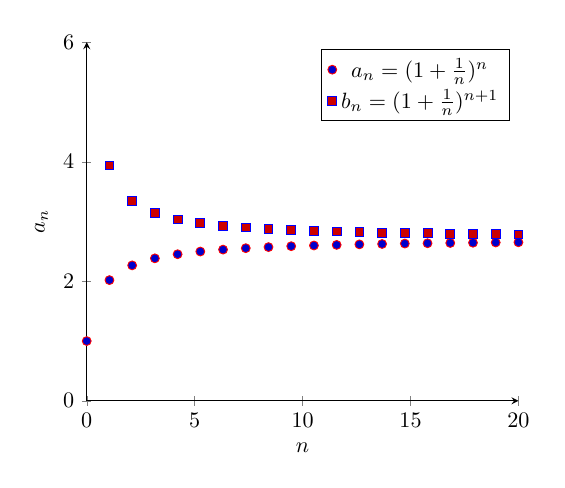
\begin{tikzpicture}[thick,scale=0.8, every node/.style={scale=1}]
\begin{axis}[
axis lines = left,
xlabel = $n$,
ylabel = {$a_n$},
ymin=0,
ymax=6,
xmin=0,
xmax=20,
]
%Below the red parabola is defined
\addplot+[only marks] [
domain=0:20, 
samples=20, 
color=red,
]
{(1+1/x)^x};
\addlegendentry{$a_n=(1 +\frac{1}{n})^n$}
\addplot+[only marks] [
domain=0:20, 
samples=20, 
color=blue,
]
{(1+1/x)^(x+1)};
\addlegendentry{$b_n=(1 +\frac{1}{n})^{n+1}$}
\end{axis}
\end{tikzpicture}

In Beispiel 1.27 werden wir sehen, dass $\lim a_n = \lim b_n$. Der Limes wird als eulersche Zahl bezeichnet. Dazu zunächst


\subsection*{1.26 Satz (Intervallschatelung)}

Seien $(a_n),(b_n)$ reelle Folgen mit
\begin{enumerate}
	\item $(a_n) \nearrow , (b_n) \searrow$
	\item $(a_n) \leq (b_n) \text{ mit } \forall n \in \mathbb{N}$
	\item $b_n - a_n \rightarrow 0$
\end{enumerate}
Dann sind $(a_n),(b_n)$ konvergent und besitzen denselben Limes. \\
(Im Beispiel oben "ziehen" beide Folgen sich zusammen um e. Klammern diesen Wert von beiden Seiten ein)\\
Beweis:\\
Es ist $a_1 \leq a_n \leq b_1 \leq b_n \text{ mit } \forall n \in \mathbb{N}$\\
\begin{enumerate}
	\item $(a_n) \nearrow$ hat obere Schranke $b_1$\\
	\item $(b_n) \nearrow$ hat untere Schranke $a_1$\\
	\item $(a_n),(b_n)$ sind konvergent.
\end{enumerate}
Da $(b_n - a_n)$ Nullfolge, sind die Grenzwerte gleich. 

\subsection*{1.27 Beispiel}
3. Bedinungen der Intervallschachtelung:\\
\begin{itemize}
	\item $(a_n) \nearrow , (b_n) \searrow$
	\item $a_n = (1+\frac{1}{n})^n \leq (1+\frac{1}{n}) *a_n = (1+\frac{1}{n})^{n+1} = b_n$ also $a_n \leq b_n$ \\
	\item $\lim b_n = \underbrace{\lim (1+ \frac{1}{n})}_{\rightarrow 1} * a_n = \lim 1 *a_n = \lim a_n$ somit $\lim b_n = \lim a_n$
\end{itemize}

\subsection*{1.28 Definition}

$$e := \lim (1+\frac{1}{n})^n = \lim (1+\frac{1}{n})^{n+1}$$

"Einführung von Teilfolgen und Häufungspunkten mit Bsp $(-1)^n$ als alternierende Folge. Sie besteht aus zwei Teilfolgen mit 1,-1. Diese sind beschränkt und konvergent. Hier wandelt Bolzano-Weierstraß unsere bisherige Deinition der Konvergenz!"


\subsection*{1.29 Bemerkung}
$(a_n)$ konvergent $\overbrace{\Rightarrow}_{1.3} (a_n)$ beschränkt. \\
Umkehrung gilt nicht! Aber $(a_n)=(-1)^n$ als Beispiel besitzt zwei konvergente Teilfolgen mit Limes +1 und -1. 

\section*{Teilfolgen und Häufungspunkte}

\subsection*{1.30 Definition: Teilfolge}
Sei $(a_n)_{n \in \mathbb{N}}$ eine Folge und $(n_k)_{k \in \mathbb{N}}$ eine streng monoton steigende Folge von Indizies. Dann heißt die Folge $(a_{n_k})$ Teilfolge von  $(a_n)_{n \in \mathbb{N}}$.\\
"Man beschränkt die Folge in Teilfolgen durch entsprechende Wahl der Indizies"


\subsection*{1.31 Beispiel}
$(a_n)=(-1)^n$
\begin{itemize}
	\item $n_k = 2k \Rightarrow a_{n_k} = a_{2k} = (-1)^{2k} = 1$ mit $k \in \mathbb{N}$\\
	\item $m_k = 2k+1 \Rightarrow a_{n_k} = a_{2k+1} = (-1)^{2k+1}= -1 $ mit  $k \in \mathbb{N}$
\end{itemize}


\subsection*{1.32 Bemerkung}
$(a_n) $ konvergent gegen a $\Rightarrow $ Jede Teilfolge konvergent gegen a


\subsection*{1.33 Definition (Häufungpunkt - HP)}
Sei $(a_n) $ reelle Teilfolge, $h\in \mathbb{R}$ heißt Häufungspunkt (HP) von $(a_n) $, wenn es eine Teilfolge von $(a_n) $ gibt, die gegen h konvergiert. 


\subsection*{1.34 Beispiel}
$(a_n) $ mit $a_n = (-1)^n + \frac{1}{n}$ hat zwei HP: $-1, +1$



\subsection*{1.35 Satz (Bolzano- Weierstraß)}
Sei $(a_n) $ reelle Folge. $(a_n) $ sei beschränkt. \\
$\Rightarrow (a_n) $ besitzt konvergente Teilfolge. \\
(Skizze: $(a_n) $  durch k beschränkt, dann muss es einen HP geben, da $(a_n) $  beschränkt und unendlich viele Folgenglieder. Sie müssen irgendwo sein ;D)\\
\textbf{Beweis:}\\
Konstruiere konvergente Teilfolge $(a_{n_k})_{k \in \mathbb{N}}$.\\
Sei $(a_n) $ beschränkt $\Rightarrow |a_n| \leq K \text{ (K geeignet wählen)}$\\
Dann folgt $a_n \in \underbrace{[-K,K]}_{sei [A_0, B_0]} \text{ mit } \forall n \in \mathbb{N}$ 
\begin{itemize}
	\item $k=1$: Halbiere das Intervall $[A_0, B_0]$.\\
	Falls in linker Hälfte unendlich viele Folgenglieder liegen, wähle eines davon aus. \\
	Falls nicht, liegen in der rechten Hälfte unendlich viele Folgenglieder. Wähle dieses aus. \\
	 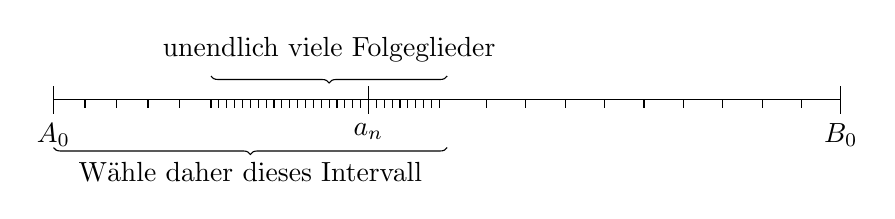
\begin{tikzpicture}[decoration=brace]
	 % Die Grundlinie:
	 \draw(0,0)--(10,0);
	 % Striche und Beschriftung in Abständen 0, 2, 4, 6, ...
	 \foreach \x/\xtext in {0/$A_0$,4/$a_n$,10/$B_0$}
	 \draw(\x,5pt)--(\x,-5pt) node[below] {\xtext};
	 % obere geschweifte Klammer mit Text darüber:
	 \draw[decorate, yshift=2ex]  (5,0) -- node[above=0.4ex] {unendlich viele Folgeglieder}  (2,0);
	 % untere geschweifte Klammer mit Text darunter:
	 \draw[decorate, yshift=-4ex] (5,0) -- node[below=0.4ex] {Wähle daher dieses Intervall} (0,0);
	 % Schleife für die kleinen Striche in Abstand, 10 pro Intervall
	 \foreach \x in {0.4,0.8,...,2}  \draw (\x,0) -- (\x,-3pt);
	 % Schleife für die kleinen Striche in Abstand, 10 pro Intervall
	 \foreach \x in {2.0,2.1,...,5}  \draw (\x,0) -- (\x,-3pt);
	 % noch so ein paar Striche in weiterem Intervall:
	 \foreach \x in {5.5,6,...,10} \draw (\x,0) -- (\x,-3pt);
	 \end{tikzpicture}\\
	 
	 Ausgewählte Folgenglieder nennen wir $a_n$, seine Intervallhälfte $[A_1,B_1]$\\
	 \item $k=2$: Halbiere $[A_1,B_1]$ und wende obiges Verfahren erneut an um $a_{n_2} \in [A_2,B_2]$ zu erhalten.
	 \item Führe Rekrusiv fort. Daraus erhält man eine Intervallschachtelung.
\end{itemize}
Es folgt:
\begin{itemize}
	\item $(A_k) \nearrow , (B_k) \searrow$
	\item $(A_k) \leq (B_k)$
	\item $(A_k -B_k) = \frac{k}{2^{k+1}} \rightarrow 0 $ (Die Intervallbreite wird immer halbiert!)
\end{itemize}
Mit 1.26 folgt nun $\lim A_k = \lim B_k$ \\
Da $A_k \leq a_{n_k} \leq B_k$ ist $\lim A_k = \lim a_{n_k}=\lim B_k$. Was zu zeigen war. 
(Hier wird die Teilfolge eingeschlossen siehe dazu auch nochmal Satz 1.15!)\\
Und $a_{n_k}$ ist konvergente Teilfolge von $(a_n)$.





\end{document}

